\section{Einleitung}

\begin{frame}
  {Determinierer und Quantifikation}
  \onslide<+->
  \onslide<+->
  Bisher haben wir nur indefinite NPs modelliert.\\
  \Zeile
  \begin{itemize}[<+->]
    \item NP-Semantik bestand nur aus Einführung eines Indexes und einer Restriktion.
    \item Was soll eine natürlichsprachliche Semantik leisten?
    \item Was haben Wahrheit (von Sätzen) und Referenz miteinander zu tun?
    \item Wie ist der semantische Beitrag von \alert{Funktionswörtern} im weiteren Sinn?
    \item Wie modelliert man Sokupsambiguitäten von Quantoren in HPSG?
  \end{itemize}
  \Zeile
  \onslide<+->
  \centering 
  \grau{\citet[47--59, Kapitel~8]{ps2} und \citet{KR2021a}}\\
\end{frame}

\section{Linguistische Theorien}

\begin{frame}
  {Bedeutung an sich ist nicht mental!}
  \onslide<+->
  \onslide<+->
  Bezug sprachlicher Zeichen zu außersprachlichen Dingen\\
  \onslide<+->
  \Zeile
  \centering 
  \begin{forest}
    [\gruen{Zeichen (Form-Bedeutungs-Paare)}
      [\gruen{Reale Objekte}, edge=gruen]
      [Mentale Konzepte]
    ]
  \end{forest}
\end{frame}

\begin{frame}
  {"`Semantik"' im generativen T-Modell}
  \onslide<+->
  \onslide<+->
  \centering 
  \resizebox{0.6\textwidth}{!}{
    \begin{tikzpicture}

      \node [rectangle, draw, align=left, color=teal, rounded corners=0.5em] (Numeration) at (5cm, -6cm) {Numeration};
      
      \node [visible on=<3->, rectangle, draw, align=left, color=gray] (Lexikon) at (1cm, -6cm) {Lexikon};
      \path (Lexikon.east) edge [visible on=<3->, line width=0.5mm, dashed] node [below, shift={(-0.4cm,0)}] {\textit{}} (Numeration.west);
     
      \node [visible on=<4->, rectangle, draw, align=left, color=gray] (Intention) at (9cm, -6cm) {Intention};
      \path (Intention.west) edge [visible on=<4->, line width=0.5mm, dashed] node [below, shift={(-0.4cm,0)}] {\textit{}} (Numeration.east);

      \node [visible on=<5->, rectangle, draw, align=left, fill=black, color=black, rounded corners=0.5em] (Syntax) at (5cm, -4.5cm) {\whyte{Syntax}};
      \path (Numeration.north) edge [visible on=<5->, line width=0.5mm, -latex] node [below, shift={(-0.4cm,0)}] {\textit{}} (Syntax.south);  

      \node [visible on=<6->, rectangle, draw, align=left, color=teal, rounded corners=0.5em] (Phrasenstruktur) at (5cm, -3cm) {Phrasenstruktur};
      \path (Syntax.north) edge [visible on=<6->, line width=0.5mm, -latex] node [below, shift={(-0.4cm,0)}] {\textit{}} (Phrasenstruktur.south);  

      \node [visible on=<7->, rectangle, draw, align=left, color=teal, rounded corners=0.5em] (PF) at (4cm, 0cm) {PF};
      \path (Phrasenstruktur.north) edge [visible on=<7->, line width=0.5mm, -latex] node [below, shift={(-0.4cm,0)}] {\textit{}} (PF.south);  
     
      \node [visible on=<8->, rectangle, draw, align=left, color=gray] (Aeusserung) at (1cm, 0cm) {Äußerung};
      \path (Aeusserung.east) edge [visible on=<8->, line width=0.5mm, dashed] node [below, shift={(-0.4cm,0)}] {\textit{}} (PF.west);
     
      \node [visible on=<9->, rectangle, draw, align=left, fill=black, color=black, rounded corners=0.5em] (Syntax2) at (6cm, -1.5cm) {\whyte{Syntax 2}};
      \path (Phrasenstruktur.north) edge [visible on=<9->, line width=0.5mm, -latex] node [below, shift={(-0.4cm,0)}] {\textit{}} (Syntax2.south);  
     
      \node [visible on=<10->, rectangle, draw, align=left, color=teal, rounded corners=0.5em] (LF) at (6cm, 0cm) {LF};
      \path (Syntax2.north) edge [visible on=<10->, line width=0.5mm, -latex] node [below, shift={(-0.4cm,0)}] {\textit{}} (LF.south);  

      \node [visible on=<11->, rectangle, draw, align=left, color=gray] (Interpretation) at (9cm, 0cm) {Interpretation};
      \path (Interpretation.west) edge [visible on=<11->, line width=0.5mm, dashed] node [below, shift={(-0.4cm,0)}] {\textit{}} (LF.east);
      
    \end{tikzpicture}
  }
\end{frame}

\begin{frame}
  {Repräsentationsebenen}
  \onslide<+->
  \onslide<+->
  Im klassischen generativen Modell:\\
  \grau{\footnotesize (In minimalistischen Modellen herrscht sowieso Anarchie.)}
  \Zeile
  \begin{itemize}[<+->]
    \item keine echte Interpretation auf LF
    \item Bewegung \rot{nachdem} der Satz geäußert wurde
    \item Herstellung einer logisch interpretierbaren \alert{Form} auf LF
    \item Grund | Generative Oberflächensyntax kann nicht alle Interpretationen abbilden
  \end{itemize}
\end{frame}


\begin{frame}
  {Richard Montague | Direkte Interpretation}
  \onslide<+->
  \onslide<+->
  Sprache ist Logik ist Sprache \ldots\\
  \Halbzeile
  \begin{itemize}[<+->]
    \item[A] Entweder ist die \alert{Übersetzung in eine LF trivial und äquivalent zur PF\slash Syntax},\\
      oder \orongsch{sie fügt etwas hinzu, das der Sprache an sich fehlt}.
    \item[B] Sätze haben aber auch \alert{mit LF-Übersetzung nur die Bedeutungen,\\
      die sie sowieso haben} \grau{(keine Hinzufügung)}.
    \item[\ding{222}] Also ist die \gruen{Übersetzung in LF trivial und äquivalent zur PF\slash Syntax}.
    \item[\ding{222}] Wir können \gruen{Sätze direkt interpretieren} (wie sie gesprochen\slash geschrieben werden).
     \Zeile 
   \item \alert{Montagues \textit{lf}} | Direkte Kodierung der Logik sprachlicher Zeichen
  \end{itemize}
\end{frame}

\section{Referentielle Semantik basal}

\begin{frame}
  {Semantische Eigenschaften von Sprache}
  \onslide<+->
  \begin{itemize}[<+->]
    \item Aussagen über die\slash Teile der Welt
    \item Ausdrücke bezeichnen\slash referieren auf Dinge i.\,w.\,S.
    \item Informativität
    \item objektiv beurteilbar (\zB Wahrheit von Sätzen)
      \Zeile
    \item \alert{Aber welche sprachlichen Einheiten referieren auf was?}
  \end{itemize}
\end{frame}

\begin{frame}
  {Referenz | Eigennamen}
  \onslide<+->
  \onslide<+->
  Ein \alert{Eigenname} \ding{222} \alert{genau ein Objekt} in der Welt\\
  \onslide<+->
  \Zeile
  \centering
    \begin{tikzpicture}
      \node [] (name) at (-6cm, 0cm) {\textit{Jan Böhmermann}};
      \node [visible on=<4->] (boehmi) at (0cm, 0cm) {
\includegraphics[width=0.2\textwidth]{\GRAPHPATH/boehmermann}};
      \path (name.east) edge [visible on=<4->, line width=0.5mm, -latex] node {\textit{}} (boehmi.west);
    \end{tikzpicture}
\end{frame}

\begin{frame}
  {Referenz | Appellativa}
  \onslide<+->
  \onslide<+->
  Ein normales \alert{Nomen} \ding{222} \alert{eine Menge von Objekten} in der Welt\\
  \onslide<+->
  \Zeile
  \centering
    \begin{tikzpicture}
      \node [] (noun) at (-6cm, 0cm) {\textit{soldier}};
      \node [visible on=<4->] (soldiers) at (0cm, 0cm) {
\includegraphics[width=0.2\textwidth]{\GRAPHPATH/soldiers}};
      \path (noun.east) edge [visible on=<4->, line width=0.5mm, -latex] node {\textit{}} (soldiers.west);
    \end{tikzpicture}
\end{frame}

\begin{frame}
  {Referenz | Adjektive und Verben}
  \onslide<+->
  \onslide<+->
  Ein (intersektives) \alert{Adjektiv} oder ein \alert{Verb} \ding{222} \alert{eine Menge von Objekten} in der Welt\\
  \onslide<+->
  \Zeile
  \centering
    \begin{tikzpicture}
      \node [] (adj) at (-6cm, 0cm) {\textit{human}};
      \node [visible on=<4->] (boehmi) at (0cm, +2cm) {
\includegraphics[width=0.1\textwidth]{\GRAPHPATH/boehmermann}};
      \path (adj.east) edge [visible on=<4->, line width=0.5mm, -latex] node {\textit{}} (boehmi.west);
      \node [visible on=<5->] (soldiers) at (0cm, 0cm) {
\includegraphics[width=0.1\textwidth]{\GRAPHPATH/soldiers}};
      \path (adj.east) edge [visible on=<5->, line width=0.5mm, -latex] node {\textit{}} (soldiers.west);
      \node [visible on=<6->] (crowd) at (0cm, -2cm) {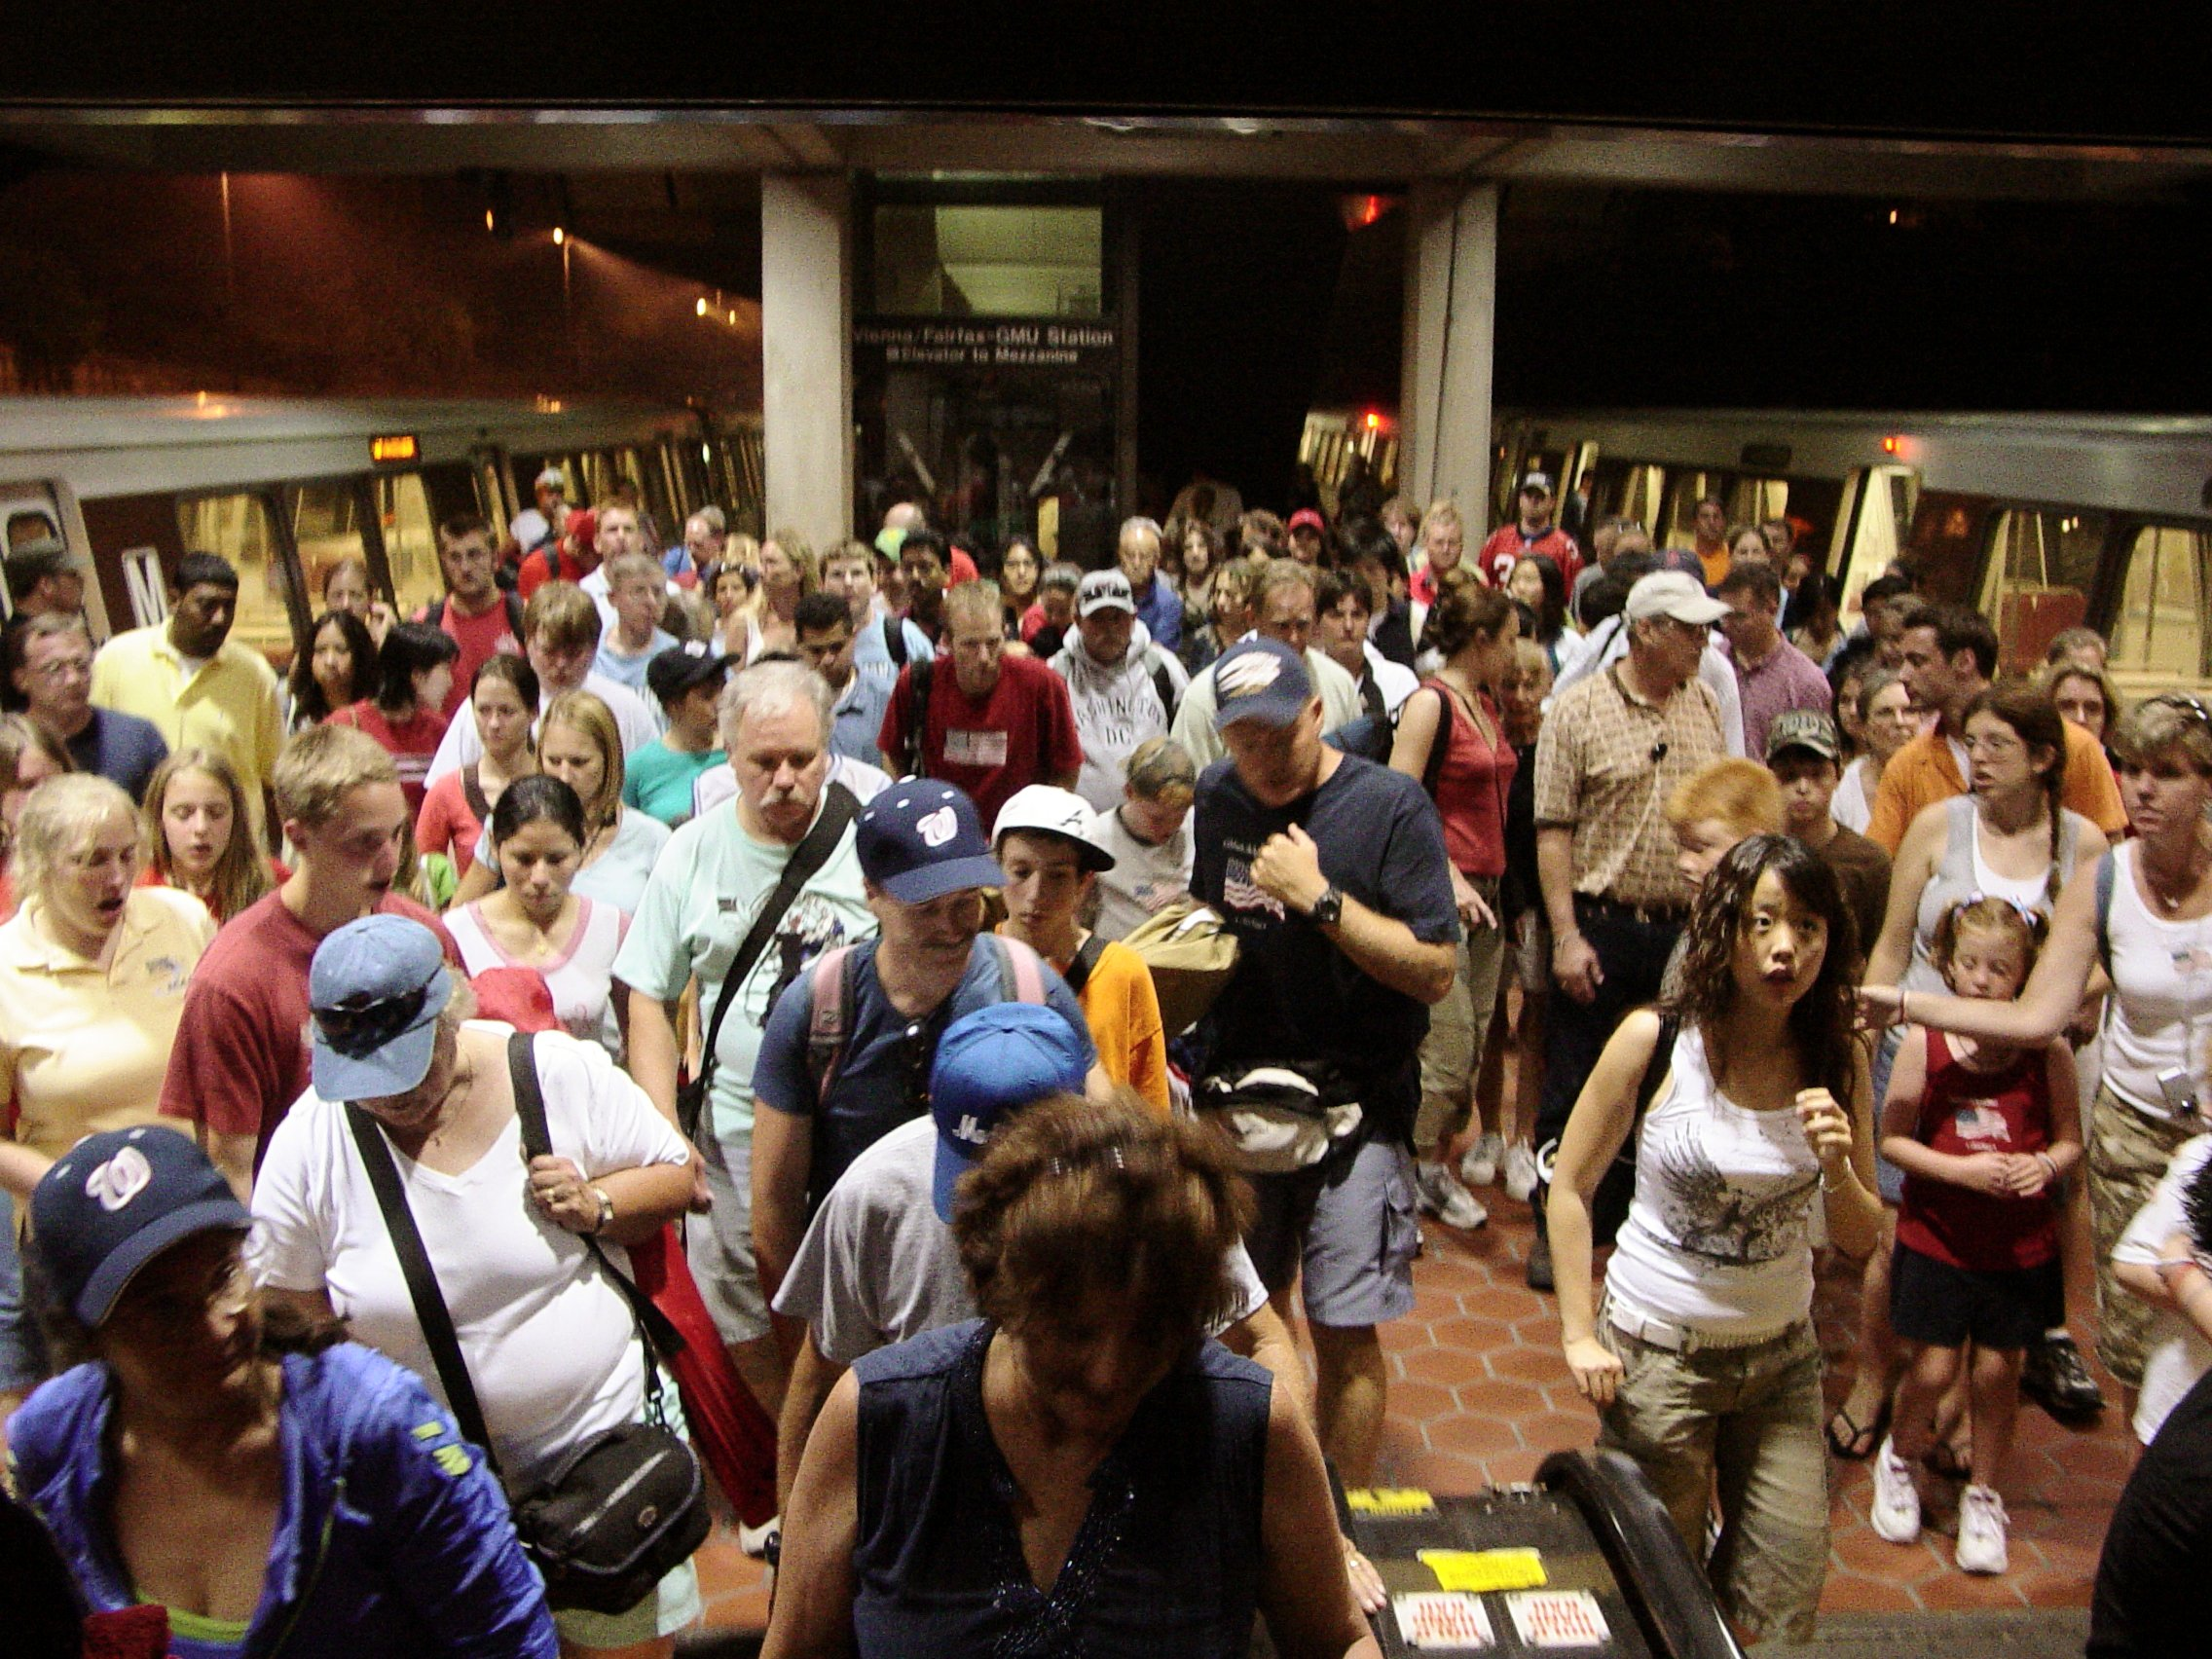
\includegraphics[width=0.1\textwidth]{\GRAPHPATH/crowd}};
      \path (adj.east) edge [visible on=<6->, line width=0.5mm, -latex] node {\textit{}} (crowd.west);
    \end{tikzpicture}
\end{frame}

\begin{frame}
  {Referenz | Sätze}
  \onslide<+->
  \onslide<+->
  Ein \alert{Satz} \ding{222} in erster Näherung \alert{ein Sachverhalt}, \alert{wahr} oder \rot{falsch}\\
  \onslide<+->
  \Zeile
  \centering
    \begin{tikzpicture}
      \node [align=left] (s) at (-6cm, 0cm) {\it A humming bird\\\it is hovering over\\\it a red flower.};

      \node [visible on=<4->, align=center] (hum) at (0cm, +2cm) {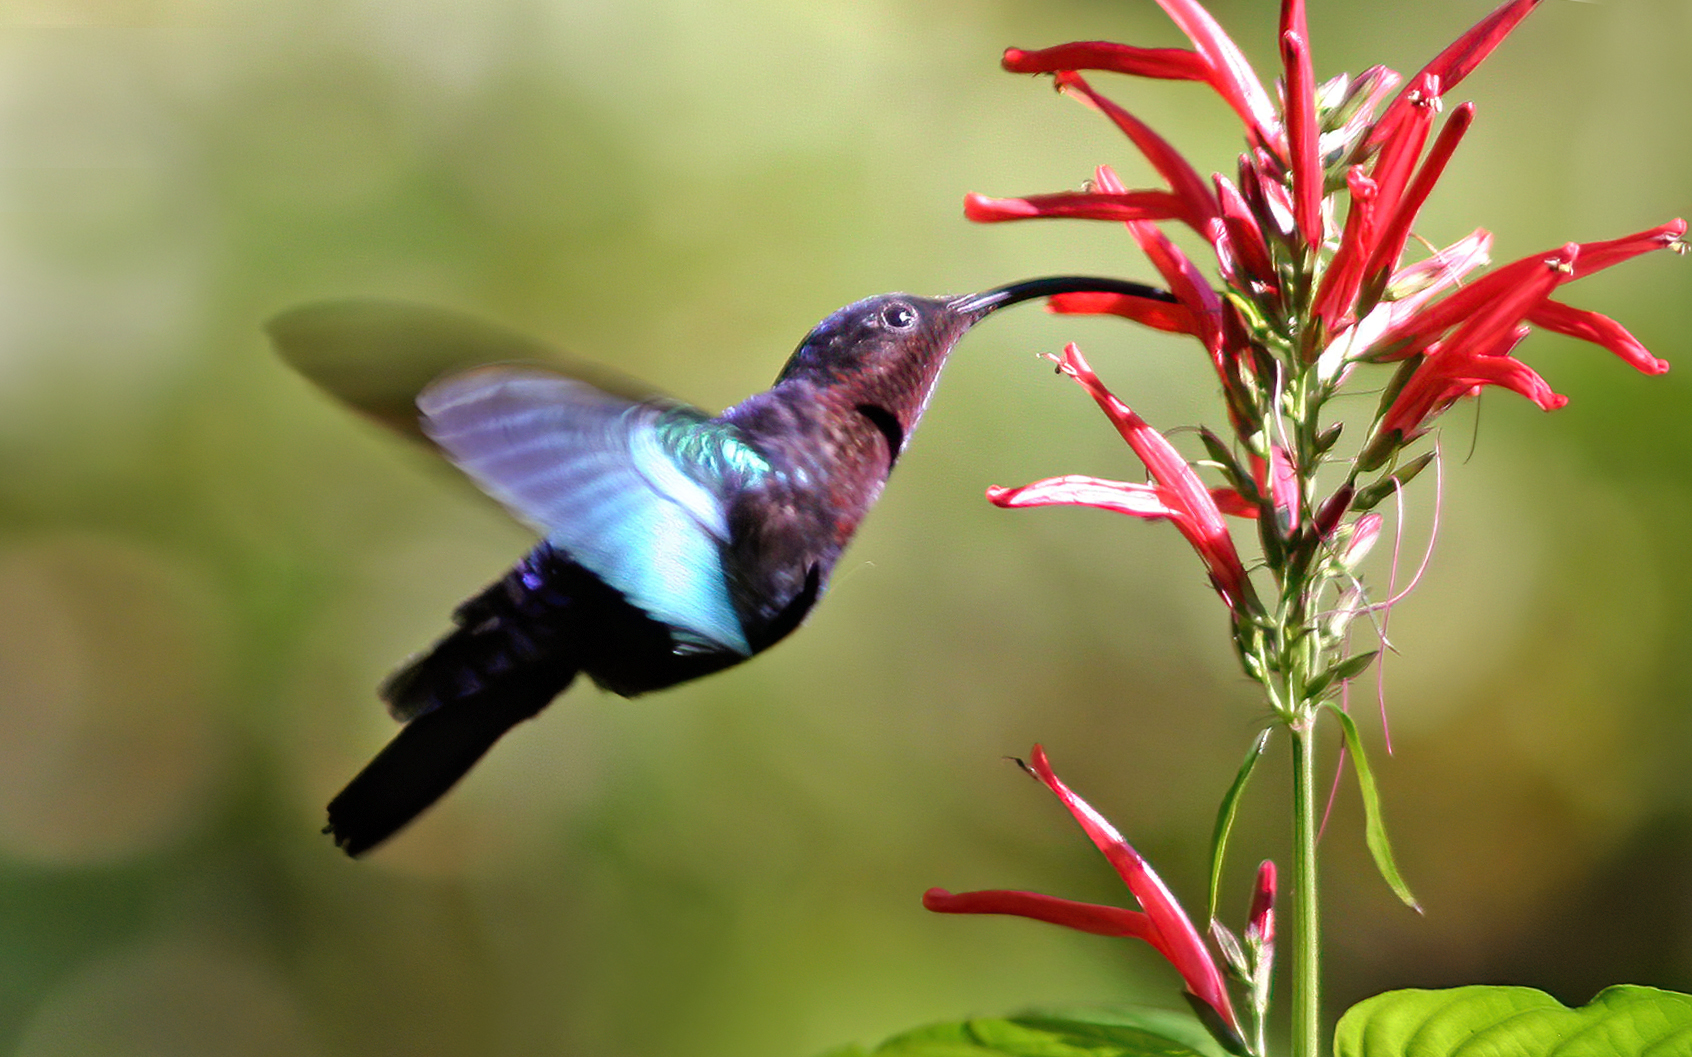
\includegraphics[width=0.2\textwidth]{\GRAPHPATH/hummingbird}};
      \path (s.east) edge [visible on=<4->, line width=0.5mm, -latex] node {\textit{}} (hum.west);
      
      \node [visible on=<5->, align=center] (boehmi) at (0cm, -2cm) {
\includegraphics[width=0.2\textwidth]{\GRAPHPATH/boehmermann}\\\footnotesize (als Individuum)};
      \path (s.east) edge [visible on=<5->, line width=0.5mm, -latex, color=red] node {\textit{}} (boehmi.west);
      \node [visible on=<6->, align=center, color=red, fill=red] (nein) at (-3.5cm, -1.25cm) {\footnotesize \whyte{Nein! falsche}\\\footnotesize \whyte{Art von Objekt}};
    \end{tikzpicture}
\end{frame}

\begin{frame}
  {Gottlob Frege | Das Frege-Prinzip}
  \onslide<+->
  \onslide<+->
  Bedeutung ist kompositional. Wir müssen das hier formalisieren:\\
  \Halbzeile
  \begin{itemize}[<+->]\small
    \item \textit{humming bird} \ding{222} die \alert{Menge} der Kolibri-Objekte
    \item \textit{a} \ding{222} \alert{Existenzaussage} für ein Element aus einer Menge
    \item \textit{a humming bird} \ding{222} \alert{Existenzaussage} für ein Element $x$\\
      aus der Menge der Kolibri-Objekte
    \item \textit{is hovering} \ding{222} die \alert{Menge} der schwebenden Objekte
    \item \textit{a humming bird is hovering} \ding{222} das existierende Kolibri-Objekt $x$\\
      ist auch ein \alert{Element der Menge} der schwebenden Objekte
    \item \textit{a red flower} \ding{222} \alert{Existenzaussage} für ein Element $y$\\
      aus der \alert{Schnittmenge} der roten Objekte und der Blumen-Objekte
    \item \textit{over} \ding{222} die \alert{Relation} zwischen Objekten (s.\ nächste Woche),\\
      die sich übereinander befinden
    \item \textit{A Humming is hovering over a red flower.} \ding{222}\\
      \gruen{Es gibt ein Objekt $x$ aus der Schnittmenge der Kolibri- und der schwebenden Objekte,\\
      und es gibt ein Objekt $y$ aus der Schnittmenge der roten und der Blumen-Objekte,\\
    und $x$ befindet sich über $y$.}
  \end{itemize}
\end{frame}

\section{Semantische Eigenschaften von Sätzen}

\begin{frame}
  {Implikation (Entailment)}
  \onslide<+->
  \onslide<+->
  Mengen von Aussagesätzen \alert{implizieren} andere Sätze.\\
  \onslide<+->
  Sätze (Implikationen) lassen sich aus anderen Sätzen (Axiome) \alert{beweisen}.\\
  \Halbzeile
  \begin{itemize}[<+->]
    \item[A] \textit{Jan Böhmermann ist ein Mensch.}
    \item[B] \textit{Jan Böhmermann ist leutselig.}
    \item[C] \textit{Jan Böhmermann ist ein leutseliger Mensch.}
      \Halbzeile
    \item[ ] \alert{$A,B\vdash C$} | A und B implizieren C. (C ist beweisbar aus A und B.)
    \item[ ] \rot{$A\not\vdash C$} | A impliziert nicht C.
    \item[ ] \rot{$B\not\vdash C$} | B impliziert nicht C.
      \Halbzeile
    \item[ ] \orongsch{$A\vdash A\wedge A$} \onslide<+->| \textit{Jan Böhmermann ist ein Mensch \orongsch{und} Jan Böhmermann ist ein Mensch.}
      \Halbzeile
    \item[D] \textit{Irgendetwas ist ein Mensch.}
    \item[ ] \alert{$A\vdash D$} 
  \end{itemize}
\end{frame}

\begin{frame}
  {Tests auf Implikation}
  \onslide<+->
  \onslide<+->
  Wenn diese Kriterien zutreffen, impliziert A B:\\
  \Zeile
  \begin{itemize}[<+->]
    \item Wenn A wahr ist, ist B auch immer wahr.
    \item Eine Situation, die von B beschrieben wird, wird auch von A beschrieben.
    \item Die Information in B ist vollständig in der Information in A enthalten.
    \item Man kann unter keinen Umständen sagen: \textit{A ist wahr, aber B ist nicht wahr.}
  \end{itemize}
\end{frame}


\begin{frame}
  {Synonymie}
  \onslide<+->
  \onslide<+->
  Synonyme Ausdrücke haben \orongsch{exakt} \alert{die gleiche Referenz}.\\
  \Halbzeile
  \begin{itemize}[<+->]
    \item Lexikalische Synonymie | \textit{humming bird} $\stackrel{lex}{\equiv}$ \textit{colibri}
      \Halbzeile
    \item Kompositionale Synonymie
      \begin{itemize}[<+->]
        \item[ ] \textit{Mulder traf seine entführte Schwester, nachdem er\\
          in die geheime Militärbasis eingebrochen war.}
        \item[$\equiv$] \textit{Bevor er seine entführte Schwester traf,\\
          brach Mulder in die geheime Militärbasis ein.}
      \end{itemize}
    \Halbzeile
    \item \alert{$A\equiv B\ \text{gdw}\ A\vdash B\ \text{und}\ B\vdash A$} (gegenseitige Implikation)
    \item \grau{\textit{gdw} = \textit{genau dann wenn} | \textit{iff} = \textit{if and only if}}
  \end{itemize}
\end{frame}


\section{Quantoren}

\begin{frame}
  {Hauptaufgaben einer formalisierten Semantik}
  \onslide<+->
  \begin{itemize}[<+->]
    \item Bedeutung von Zeichen modellieren
    \item Bedeutung = Bezug zur Welt = Wahrheitsbedingungen (bei Sätzen)
    \item Relationen zwischen Zeichen (Implikation, Synonymie usw.) modellieren
      \Halbzeile
    \item \alert{Funktionswörter} im weitesten Sinn erklären, unter anderem:
    \item Quantoren | \textit{drei Kolibris}, \textit{alle Bücher}, \textit{wenige Kollegen} usw.
      \begin{itemize}[<+->]
        \item Nicht durch Zeigen und Vormachen erklärbar
        \item Trotzdem klarer Bezug zur Welt\\
          \grau{\footnotesize Alle Bücher gehören drei Kollegen.}
        \item Führen zu \alert{Ambiguitäten}
      \end{itemize}
  \end{itemize}
\end{frame}

\begin{frame}
  {Skopus}
  \onslide<+->
  \onslide<+->
  Skopusambiguitäten\\
  \Zeile 
  \begin{itemize}[<+->]
    \item[ ] \textit{Einen Linguisten mögen alle Menschen.}
      \Zeile
    \item[A] Für \alert{alle} \gruen{Menschen} {\footnotesize\mybox{1}} : [ Es gibt \alert{einen} \gruen{Linguisten} {\footnotesize\mybox{2}} : [ {\footnotesize\mybox{1}} \gruen{mag} {\footnotesize\mybox{2}} ] ]
    \item[B] Es gibt \alert{einen} \gruen{Linguisten} {\footnotesize\mybox{2}} : [ Für \alert{alle} \gruen{Menschen} {\footnotesize\mybox{1}} : [ {\footnotesize\mybox{1}} \gruen{mag} {\footnotesize\mybox{2}} ] ]
    \item[~] \grau{\footnotesize Man kann Quantor-Skopus-Strukturen lesen wie eine Anweisung der Auswertung der Sätze.}
      \Zeile
    \item Wie können diese mehreren Lesarten eines Satzes abgebildet werden?
    \item In GB mittels LF-Bewegung der Quantoren-NPs
    \item In HPSG unter anderem Mittels \alert{Quantorenspeicher} \grau{\citet{Cooper83}}
  \end{itemize}
\end{frame}

\section{Quantorenspeicher in HPSG}

\begin{frame}
  {Situationssemantik und Wahrheit}
  \onslide<+->
  \onslide<+->
  Situationssemantik \alert{beschreibt Situationen}.\\
  \Halbzeile
  \begin{itemize}[<+->]
    \item \alert{Satz} | Beschreibung einer \alert{Situation} (psoa).
    \item \alert{Nomen}, \alert{Adjektiv} | \alert{Objektbezug} (\textsc{index}) und \alert{Einschränkung} (\textsc{restriction})
    \item \alert{Verb} | \alert{Art der Situation} (\textit{relation}) mit \alert{Objektbezug} und \alert{Rollen}
    \item \alert{Quantoren} (\textit{alle}, \textit{einige}, \textit{zwei} usw.) | Siehe unten!
      \Halbzeile
    \item \alert{Wahrheit}
      \begin{itemize}[<+->]
        \item In klassischen Prädikatenlogiken Grundlage der Satzbedeutung
        \item In Situationssemantik sekundär
        \item Wahrheit mittels Abgleich zwischen Situationsbeschreibung und Realität
      \end{itemize}
  \end{itemize}
\end{frame}

\begin{frame}
  {Quantorenspeicher}
  \onslide<+->
  \onslide<+->
  Quantorenausdrücke bringen eine Quantorenstruktur \alert{im Speicher} mit. AVM für \textit{alle}:\\
  \onslide<+->
  \Halbzeile
  \centering 
  \scalebox{0.7}{\begin{avm}
    \[
      phon & \phon{alle} \\
      synsem|loc & \[
        cat|head|\orongsch{spec} & \[ loc|cont|nucleus & \@2 \]\\
        cont|nucleus & \@5 \[ \asort{all-quant} 
%          det & \textit{all-quant} \\
          \gruen{restind} & \gruen{\@2} \\
        \] \\
      \] \\
      \alert{qstore} & \alert{\{\@5\}} \\
    \]
  \end{avm}}\\
  \Halbzeile
  \begin{itemize}[<+->]
    \item \textsc{cont} hat jetzt \textsc{quants} und \textsc{nucleus}.
    \item Bei nicht-quantifizierten Zeichen ist \textsc{nucleus} wie \textsc{cont} bisher mit \textsc{ind} und \textsc{restr}.
    \item Bei einem Determinierer hat er einen quantorspezifischen Subtyp und \textsc{restind}.
    \item Ein \gruen{\textsc{restind}} ist ein restringierter Index, der den \textsc{nuc} des N-Kopfs nimmt.
    \item Mit Determinierer-Subtyp und der N-Bedeutung (z.\,B.\ \textit{Mensch}): \blau{\textit{Für alle Menschen}}.
    \item Der \alert{\textsc{qstore}} ist eine \alert{Menge} von solchen Quantorenausdrücken.
    \item Bereits im Lexikon: Der Quantor ist im Speicher, muss also noch Skopus nehmen.
  \end{itemize}
\end{frame}

\begin{frame}
  {NP-Bedeutung}
  \onslide<+->
  \onslide<+->
  Für \textit{alle Menschen}:\\
  \onslide<+->
  \Zeile
  \centering 
  \scalebox{0.7}{\begin{avm}
      \[
        phon & \phon{alle,Menschen} \\
        synsem|loc|cont & \[
          quants & \<\> \\
          nuc & \@2 \[
            ind & \@1 \[ num & pl \] \\
            restr & \<\[ \asort{human-rel}
              inst & \@1 \\
            \]\>
          \] \\
        \] \\
        qstore & \{\[ \asort{all-quant} 
          restind & \@2 \\
        \]\}
      \]
    \end{avm}
  }\\
  \Halbzeile
  \begin{itemize}[<+->]
    \item \textsc{qstore} muss irgendwie aufgesammelt werden.
    \item Der semantische Beitrag der NP bleibt wie bisher (bis auf \textsc{nuc}).
    \item Genial: Verbindung der NP mit dem Verb funktioniert wie bisher.
  \end{itemize}
\end{frame}

\begin{frame}
  {Andere NP}
  \onslide<+->
  \onslide<+->
  Für \textit{einen Linguisten}:\\
  \onslide<+->
  \Zeile
  \centering 
  \scalebox{0.7}{\begin{avm}
      \[
        phon & \phon{einen,Linguisten} \\
        synsem|loc|cont & \[
          quants & \<\> \\
          nuc & \@2 \[
            ind & \@1 \[ num & sg \] \\
            restr & \<\[ \asort{linguist-rel}
              inst & \@1 \\
            \]\>
          \] \\
        \] \\
        qstore & \{\[ \asort{some-quant} 
          restind & \@2 \\
        \]\}
      \]
    \end{avm}
  }\\
\end{frame}

\begin{frame}
  {VP-Bedeutung I}
  \onslide<+->
  \onslide<+->
  Für \textit{mögen einen Linguisten} (ohne Bewegung):\\
  \onslide<+->
  \Zeile
  \centering 
  \scalebox{0.7}{
    \begin{avm}
      \[
        phon & \phon{mögen,einen,Linguisten} \\
        snysem|loc|cont & \[
          quants & \<\> \\
          nuc & \@1 \[
            restr & \<\[ \asort{like-rel}
              agent & \textit{index} \\
              other & \@2 \\
            \]\>
          \]
        \] \\
        qstore & \{\[ \asort{some-quant} 
          restind & \[
            ind & \@2 \[ num & sg \] \\
            restr & \<\[ \asort{linguist-rel}
              inst & \@2 \\
            \]\>
          \] \\
        \]\}
      \]
    \end{avm}
  }
\end{frame}

\begin{frame}
  {VP-Bedeutung II}
  \onslide<+->
  \onslide<+->
  Für \textit{Alle Menschen mögen einen Linguisten} (ohne Bewegung):\\
  \onslide<+->
  \Zeile
  \centering 
  \scalebox{0.7}{
    \begin{avm}
      \[
        phon & \phon{alle,Menschen,mögen,einen,Linguisten} \\
        snysem|loc|cont & \[
          quants & \<\> \\
          nuc & \@1 \[
            restr & \<\[ \asort{like-rel}
              agent & \@3 \\
              other & \@2 \\
            \]\>
          \]
        \] \\
        qstore & \{\[ \asort{some-quant} 
          restind & \[
            ind & \@2 \[ num & sg \] \\
            restr & \<\[ \asort{linguist-rel}
              inst & \@2 \\
            \]\>
          \] \\
        \],\[
          \asort{all-quant} 
          restind & \[
            ind & \@3 \[ num & pl \] \\
            restr & \<\[ \asort{human-rel}
              inst & \@3 \\
            \]\>
          \] \\
        \]
      \}
      \]
    \end{avm}
  }
\end{frame}

\begin{frame}
  {Skopusnahme I}
  \onslide<+->
  \onslide<+->
  Um alle Lesarten zu erzeugen, setzen \citet[Kapitel~8]{ps2}\\
  Beschränkungen auf das \alert{Leeren} des \textsc{qstore}.\\
  \onslide<+->
  \Zeile
  \centering 
  \scalebox{0.6}{
    \begin{avm}
      \[
        phon & \phon{alle,Menschen,mögen,einen,Linguisten} \\
        snysem|loc|cont & \[
          \alert{quants} & \alert{\@4}\rot{$\oplus$\@5} \\
          nuc & \@1 \[
            restr & \<\[ \asort{like-rel}
              agent & \@3 \\
              other & \@2 \\
            \]\>
          \]
        \] \\
        \orongsch{qstore} & \orongsch{\{\}} \\
      \alert{retrieved} & \alert{\@4 \<
        \[ \asort{some-quant} 
          restind & \[
            ind & \@2 \[ num & sg \] \\
            restr & \<\[ \asort{linguist-rel}
              inst & \@2 \\
            \]\>
          \] \\
        \],
        \[
          \asort{all-quant} 
          restind & \[
            ind & \@3 \[ num & pl \] \\
            restr & \<\[ \asort{human-rel}
              inst & \@3 \\
            \]\>
          \] \\
        \]
      \>} \\
      \rot{hd-dtr} & \rot{\[ snysem|loc|cont|quants & \@5 \]} \\
      \]
    \end{avm}
  }
\end{frame}

\begin{frame}
  {Skopusnahme II}
  \onslide<+->
  \onslide<+->
  Genau so möglich:\\
  \grau{\footnotesize Hinweis: Die Leerung muss nicht am obersten Knoten und auch nicht auf einmal geschehen.}\\
  \onslide<+->
  \Zeile
  \centering 
  \scalebox{0.6}{
    \begin{avm}
      \[
        phon & \phon{alle,Menschen,mögen,einen,Linguisten} \\
        snysem|loc|cont & \[
          \alert{quants} & \alert{\@4}\rot{$\oplus$\@5} \\
          nuc & \@1 \[
            restr & \<\[ \asort{like-rel}
              agent & \@3 \\
              other & \@2 \\
            \]\>
          \]
        \] \\
        \orongsch{qstore} & \orongsch{\{\}} \\
      \alert{retrieved} & \alert{\@4 \<
        \[
          \asort{all-quant} 
          restind & \[
            ind & \@3 \[ num & pl \] \\
            restr & \<\[ \asort{human-rel}
              inst & \@3 \\
            \]\>
          \] \\
        \]
        \[ \asort{some-quant} 
          restind & \[
            ind & \@2 \[ num & sg \] \\
            restr & \<\[ \asort{linguist-rel}
              inst & \@2 \\
            \]\>
          \] \\
        \]
      \>} \\
      \rot{hd-dtr} & \rot{\[ snysem|loc|cont|quants & \@5 \]} \\
      \]
    \end{avm}
  }
\end{frame}


\begin{frame}
  {Quantifier Inheritance Princriple}
  \onslide<+->
  \onslide<+->
  \centering
  \Zeile
  Der \textsc{qstore} einer Phrase ist die Vereinigungsmenge der \textsc{qstore} der Töchter\\
  ohne diejenigen Einträge, die an der Phrase auf \textsc{retrieved} stehen.
\end{frame}

\begin{frame}
  {Semantics Principle für \textit{headed-phrase} (vereinfacht)}
  \onslide<+->
  \onslide<+->
  \centering 
  \Zeile
  a.~Der \textsc{qstore} einer Phrase ist die Vereinigung der \textsc{qstore}-Mengen der Töchter\\
  der Phrase abzüglich der Elemente, die auf der \textsc{retrieved}-Liste stehen.\\
  \onslide<+->
  \Zeile
  b.~\alert{Falls} der \textsc{cont} des Kopfs quantifikational ist, ist der \textsc{nuc} der Phrase identisch\\
  mit dem \textsc{nuc} des Kopfs, und der \textsc{quant}-Wert der Phrase ist die Konkatenation\\
  von \textsc{retrieved} und dem \textsc{quants} des Kopfs.\\
  \onslide<+->
  \Halbzeile
  \alert{Andernfalls} muss \textsc{retrieved} leer sein, und der \textsc{cont} des Kopfs ist\\
  gleich dem \textsc{cont} der Phrase.
\end{frame}

\section{Nächste Woche}

\begin{frame}
  {Vorbereitung}
  \centering 
  \large
  Nächste Woche reden wir über Unterspezifikationssemantik.\\
  \Zeile
  \rot{Sie sollten dringend vorher aus \citet{CFPS2005a}\\
  die Seiten 281--291 und 304--311 lesen (s.~Webseite)!}\\
  \Viertelzeile
  Das sind \rot{18} Seiten.\\
\end{frame}
